%----------------------------------------------------------------------------------------
%	PACKAGES AND DOCUMENT CONFIGURATIONS
%----------------------------------------------------------------------------------------
\documentclass[a4paper, 12pt]{article}

%\documentclass{article}

\usepackage{graphicx} % Required for the inclusion of images
%\usepackage{natbib} % Required to change bibliography style to APA
\usepackage{amsmath} % Required for some math elements 

\setlength\parindent{0pt} % Removes all indentation from paragraphs

\renewcommand{\labelenumi}{\alph{enumi}.} % Make numbering in the enumerate environment by letter rather than number (e.g. section 6)

%\usepackage{times} % Uncomment to use the Times New Roman font


%\usepackage[latin1]{inputenc}

\usepackage{amsmath, amssymb}

\usepackage[finnish]{babel}
\usepackage[utf8x]{inputenc}
\usepackage{fancyhdr}
\usepackage{listings}


\usepackage{listings}
\usepackage{color}

\usepackage{graphicx}
\usepackage{hyperref}
\usepackage{wrapfig}
\usepackage{lscape}
\usepackage{rotating}
\usepackage{epstopdf}
\usepackage[numbers]{natbib}
 
\lstset{ %
  backgroundcolor=\color{white},
  basicstyle=\footnotesize,
  language=Java,
  tabsize=2
}

%----------------------------------------------------------------------------------------
%	DOCUMENT INFORMATION
%----------------------------------------------------------------------------------------

\title{Säteilyn ilmaisin} % Title

\author{Alexey \textsc{Sofiev}} % Author name

\date{19.05.2016} % Date for the report

\begin{document}

\maketitle % Insert the title, author and date

\begin{center}
\begin{tabular}{l r}
Suorituspäivä: & 18 Toukokuuta, 2016 \\ % Date the experiment was performed
Työpari: & Tudor Florea \\ % Partner names
& Jari Honko \\
Opiskelijanumeroni: & 013573003 % Instructor/supervisor
\end{tabular}
\end{center}

\clearpage
\section{Tiivistelmä}

Fysiikan aineopintojen toisen laboratoriotyön tarkoituksena oli rakentaa tuikeilmaisin havaitsemaan gammasäteilyä. Päätehtävänä oli tutustua tuikeilmaisimen toimintaan ja siinä hyödynnettävään elektroniikkaan. Lisätehtävänä oli tutkia säteilyn vaimenemista lyijyssä.

Molemmat tehtävät onnistuivat, määritetty lyijyn vaimenemiskerroin vastaa teoreettista tilannetta virherajojen sisällä. Huolimatta laitteiston suunnitellusta toiminnallisuudesta, virherajoissa on yhä pienentämistä.

\clearpage

\section{Johdanto}

Tämän laboratoriotyön tarkoituksena oli rakentaa laitteisto, joka pystyisi havaitsemaan gammasäteilyä. Työssä on valittu havainnointikappaleeksi tuikekide, joka muuntaa siihen osuvaa gammasäteilyä valon tuikahdukseksi. Saatu signaali on kuitenkin hieman heikko, joten ennen sen rekisteröintiä se päästetään valomonistinputkesta läpi (PMT, photomultiplier tube), jonka jälkeen voimistunut valosignaali kerätään ja muutetaan sähköiseksi signaaliksi. Muuttaminen tapahtuu esivahvistimen avulla. Saatu signaali ohjataan tietokoneen äänikortille, josta se kerätään talteen PRA11 ohjelman avulla.

Ennen varsinaista mittausta tutkitiin rakennetun piirin ulostulevan signaalin muotoja oskilloskoopilla, mm. esivahvistin ja vahvistin.

Mittaukset aloitettiin taustasäteilyn mittauksella, jotta sitä voitaisiin poistaa analyysivaiheessa. Säteilyn lähteenä oli Cs-137, ja se oli asetettu parin cm korkeudelle lähteestä. Gammasäteilyn vaimenemista lyijyssä tutkittiin lisämällä ohuita 0.13 -- 0.16 cm paksuisia levyjä säteilylähteen ja tuikeilmaisimen väliin.

\section{Koejärjestely}
\subsection{Koejärjestely yleisesti}
Kuva 1 kuvaa koejärjestelyä. 

\begin{figure}[!hbt]
\includegraphics[scale=0.7]{Koejarjestely}
\label{fig:Koejarjestely}
\caption{Kaaviokuva koejärjestelystä. Jännitelähde tuotti 28V:n jännitettä. Lähde: \cite{TyoMoniste}}
\end{figure}

Kuten mainittiin Johdannossa, tarkoituksena on että säteilylähteeltä tulevaa säteilyä osuu tuikeilmaisimeen ja muuttuu valoksi, jota voimistetaan valomonistinputkella (SiPM). Sen jälkeen signaali muutetaan sähköiseksi ja vahvistetaan (Esivahvistin ja vahvistin), jonka jälkeen se kulkeutuu tietokoneen äänikortin kautta PRA11-ohjelmalle.(PC)

Helpottaakseen laitteiston rakentamista laboratorio-olosuhteissa Kuva 2 näyttää miltä laitteiston osat näyttävät luonnossa.

\begin{figure}[!hbt]
\includegraphics[scale=0.9]{LaitteistonOsat}
\label{fig:LaitteistonOsat}
\caption{Laitteiston osat. 1. Valoanturi, jonka vihreän osan päällä on tuikekide; 2. Esivahvistin; 3.Vahvistin; 4. Mittaustilanne, jossa on suljettu valoanturi ja 2 lyijylevyä päällä.}
\end{figure}

Kuvan 2 ensimmäisessä kuvassa on auki oleva valoanturi, jonka vihreän osan keskellä on läpinäkyvä tuikeilmaisin. Mittausten aikana tuo laatikko on kiinni, jotta vältetään näkyvän valon häiriötä. Toisessa kuvassa (oikea ylänurkka) on esivahvistin. Kolmannessa vahvistin, ja neljännessä kuvassa on kuva mittaustilanteesta, jossa on statiivilla kiinni säteilyn lähde, valoilmaisin suljettu, sekä säteilyn lähteen ja tuikeilmaisimen välissä on lyijylevy vaimentamassa. Lisäksi neljännessä kuvassa on mittausväline, jolla määritetään levyjen paksuus. (eivät olleet tasapaksuja)

\subsection*{Häiriötekijät ja ratkaisut}
\paragraph{Ulkoinen valo\\}
Ulkoinen valo on huomattavasti suurempi kuin tuikekiteestä saatava signaali, joten valoanturi on suljettu mustaan ei-läpinäkyvään laatikkoon.

\paragraph{Tuikekiteen paikkariippuvuus\\}
Tuikekide on vain seisomassa anturin paikalla, joten on tönäisyherkkä, ja sen pienehkönkin liikahduksen on havaittu muuttavan tuloksia suuresti. Pienentääkseen liikahtamista musta laatikko teipattiin kiinni pöytään. Huomautus: jos liian pieni signaali, niin se johtuu siitä, että kide on pois paikaltaan.

\paragraph{Taustakohina\\}
Taustasäteilyä ei ollut mahdollista eliminoida laboratorio-oloissa, joten sitä yritetään pienentää kahdella tavalla: 1) suodattamalla liian heikon signaali pois, ja 2) mittaamalla tausta ja vähentämällä sen tutkimustuloksista.

\section{Teoria}

Tarkasteltaessa säteilylähteen intesiteettiä, on huomioitavaa kolme tekijää:
\begin{enumerate}
\item[1] Säteilyaineen puoliintumista ajan myötä.
\item[2] Säteilyn jakautuminen kaikkiin suuntiin, joten tarkastelusuuntaan tulee vain osa säteilystä.
\item[3] Säteilyn vaimeneminen väliaineessa.
\end{enumerate}

Tässä työssä ei ole tavoitteena määrittää lähteen aktiivisuus, vaan tutkia säteilyn käyttäytymistä väliaineessa, joten kohdat 1-2 voi jättää huomiotta. Lisäksi ilmassa vaimeneminen on pientä vertaen lyijyyn \cite{GammaLead} \cite{GammaAir}, joten vaimeneminen ilmassa voidaan jättää huomiotta.

\subsection{Gammasäteilyn vaimeneminen}

Säteilyn laki noudattaa eksponentiaalista vaimenemista väliaineessa \cite{Vaimeneminen}
\begin{equation}
I = I_0 * e^{\mu x}
\label{eq:SateilynVaimeneminen}
\end{equation}
Jossa I on intensiteetti, $I_0$ on alkuperäinen voimakkuus, $\mu$ on vaimenemiskerroin, ja x on matka väliaineessa.

Kun x on hallittavissa ja I on mitattavissa, niin tutkitaan kahden tapauksen erotusta ja otetaan logaritmi Kaavasta \ref{eq:SateilynVaimeneminen}, jolloin saadaan Kaava \ref{eq:logSateilynVaimeneminen}:

\begin{equation}
log(I_n - I_{n-1}) = log(I_0) + {\mu (x_n - x_{n-1})}
\label{eq:logSateilynVaimeneminen}
\end{equation}

Eli suoran sovituksella ($\triangle x$, $log(\triangle I)$)-koordinaatistossa saadaan selville levyjen vaimenemiskertoimet.

\subsection{Virheen arviointi}
\subsubsection{Taustan poisto}
Taustamittauksesta lasketaan kuinka monta tuikahdusta aiheutuu sekunnittain. Tämä keskiarvo poistetaan jokaisesta mittauksesta.

\subsubsection{Otoksen virhe}
Taustavähennetyssä datasta lasketaan mittauksen epävarmuutta hyödyntäen otosvarianssi.

\begin{equation}
s^2 = \dfrac{1}{N-1} \sum_i (y_i - y)^2 
\label{eq:otosvarianssi}
\end{equation}
Jossa $s^2$ on otosvarianssi, $y_i$ mittaustulos, y keskiarvo, N mittausten lukumäärä.

Jolloin mittausvirhe on

\begin{equation}
s_x=s/\sqrt{N}
\label{eq:mittausVirhe}
\end{equation}

\subsubsection{Virheen kasautumislaki}
Taustan ja mittauksen virheiden yhdistynyttä tulosta lasketaan virheen kasautumislailla, eli Kaava \ref{eq:kasautumislaki}:

\begin{equation}
\sigma_{mittaus+tausta}^2 = \sigma_{mittaus}^2 + \sigma_{tausta}^2  
\label{eq:kasautumislaki}
\end{equation}

Nyt hieman tarkastellaan tapaustamme. Tarkastelemme mittauksen epätarkkuutta, eli $log(I+\sigma)$

\begin{equation}
log(I+\sigma)=log(I(1+\sigma /I))=log I + log(1+\sigma /I)
\label{eq:logJohto1}
\end{equation}

Nyt approximoidaan tämä (Kaava \ref{eq:logJohto1}) Taylorin sarjan ensimmäisillä polynomeilla, jolloin saadaan Kaava \ref{eq:logJohto2}:

\begin{equation}
log(I+\sigma)=log I + log(1+\sigma /I) \approx log(I) + \sigma /I
\label{eq:logJohto2}
\end{equation}
Kun I on huomattavasti suurempi kuin $\sigma$, eli meidän tapauksessa. Näin olleen Kaavasta \ref{eq:logJohto2} saadaan y-akselin virhepylväät (log($\triangle I$), $\triangle x$) kuvaajalle, joka on kasautumislain virhe jaettuna signaalin voimakkuudella. 

\section{Mittaus}
Mittaus on hyvä aloittaa tarkistamalla että laitteisto toimii.
\subsection{Esivahvistimen signaali}

Kuva 3 näyttää esivahvistimen signaalia. Mitattu signaali vastaa teoriata.

\begin{figure}[!hbt]
\includegraphics[scale=1.2]{EsivahvistinSignaali}
\label{fig:EsivahvistimenSignaali}
\caption{Esivahvistimen signaali. Saatu pulssi vastaa teoriaa. \cite{TyoMoniste}}
\end{figure}


\subsection{Vahvistimen signaali}
Kuva 4 näyttää vahvistimen signaalia. Mitattu signaali vastaa teoriata.
\begin{figure}[!hbt]
\includegraphics[scale=1.2]{VahvistinSignaali}
\label{fig:VahvistimenSignaali}
\caption{Vahvistimen signaali. Saatu pulssi vastaa teoriaa. \cite{TyoMoniste}}
\end{figure}

\subsection{Taustan heikon signaalin suodatus}
Tutkimus aloitetaan mittaamalla taustaa, ja sitten tuomalla säteilylähteen lähelle, jolloin histogrammisesti havaitaan mielenkiintoalue. Kuva 5 esittelee mittauksemme suodatusarvon löytämistä.

\begin{figure}[!hbt]
\includegraphics[scale=0.5]{CuttingHistogram}
\label{fig:Cutting}
\caption{Heikon taustakohinan poisto}
\end{figure}

Säteilijän signaali on Poisson/Gaussisesti jakautunut, sillä välin kun kohina on eksponentiaalinen, joten yritetään valita sellainen arvo, joka poistaisi mahdollisimman paljon taustaa, ja suhteellisen vähän siihen verrattuna säteilijän signaalia. Työssämme arvo 4 on osoittautunut hyväksi kynnykseksi.

\section{Tulokset}

Käyttäen edellä mainittua teoriaa ja mitattua datajoukkoa, saadaan Kuva 6.

\begin{sidewaysfigure}[!hbt]
\includegraphics[scale=0.45]{../SateilynVaimeneminen}
\label{fig:SateilynVaimeneminen}
\caption{Säteilyn vaimeneminen}
\end{sidewaysfigure}

Käytetty säteilijä on pääosin Cs-137, jonka säteilyn energia on 661.64 keV. \cite{CsEnergy}. Lyijyn tiheys on 11.34 * $10^3$ kg/$m^3$ ja absortiokerroin per tiheys ($\sigma/\rho$) edellä mainitulle energialle on noin 467.2 $cm^2/g$ \cite{GammaLead} eli saadaan 

\begin{equation}
\mu = 467.2 *10^4 m^2 / 10^{-3} kg / 11.34 *10^3 kg/m^3  \approx 0.412\ \ 1/mm
\end{equation}

Eli teoreettinen arvo on mittausvirheen sisällä saadusta arvosta.

\section{Johtopäätökset}

Mittauslaitteiston rakentaminen onnistui, mittauksissa saatu arvo lyijyn vaimentamiskertoimelle on teoreettisen arvion sisällä. Suoran sovitus tuotti suuria parametrien virheitä, jotka ainakin silmämääräisesti eniten johtuivat ensimmäisestä mittauksesta ilman lyijykerrosta.

Selityksenä sille voidaan olettaa, että jopa ohut lyijykerros suodattaa jonkun energiaspektrin taustasäteilystä pois, jolloin suojakerroksen olemassaololla ja puutteella on suurta eroa.

\clearpage
\section{Viitteet}

\begin{thebibliography}{1}

\bibitem{TyoMoniste} AOL 1.2 Työmoniste 2016, Tiiviskurssi, \url{https://moodle.helsinki.fi/pluginfile.php/1228493/mod_resource/content/3/AOLI.2.S%C3%A4teilyn_ilmaisin.pdf}, katsottu 20160519

\bibitem{Vaimeneminen} \url{http://www.nuclear-power.net/nuclear-power/reactor-physics/interaction-radiation-matter/interaction-gamma-radiation-matter/gamma-ray-attenuation/}, katsottu 20160519. 

\bibitem{GammaLead} \url{http://physics.nist.gov/PhysRefData/XrayMassCoef/ElemTab/z82.html}, katsottu 20160519.

\bibitem{GammaAir} \url{http://physics.nist.gov/PhysRefData/XrayMassCoef/ComTab/air.html}, katsottu 20160519.

\bibitem{CsEnergy} \url{https://www.cpp.edu/~pbsiegel/bio431/genergies.html}, katsottu 20160519.

\end{thebibliography}

\section{Liitteet}
Mittauspöytäkirjat, analysointiskriptit yms:
\url{https://github.com/AleksDark/TiivisLabrat/tree/master/2GammasateilynVaimeneminen}

\end{document}
